\begin{figure}[H]
\centering
\begin{forest}
for tree={
    draw,
    rounded corners,
    align=center,
    minimum width=2.6cm,
    minimum height=1cm,
    inner sep=4pt,
    font=\small,
    edge={-Latex}
},
selected/.style={fill=blue!10},
good/.style={fill=green!20},
bad/.style={fill=red!20},
local/.style={fill=yellow!15},
edge label/.style={midway, sloped, font=\scriptsize}
%
% ---------------- TREE ----------------
[Node $P_0$\\Local solver state\\{\scriptsize LP sol., bounds}
    [Branch on $x_i \le 0$, good,
        edge label={node[midway,above]{local policy}}
    ]
    [Branch on $x_i \ge 1$, selected,
        edge label={node[midway,above]{local policy}}
        [Node $P_1$\\Local solver state\\{\scriptsize LP sol., bounds}
            [Pruned, bad,
                edge label={node[midway,above]{bound}}
            ]
            [Feasible, good,
                edge label={node[midway,above]{solution}}
            ]
        ]
    ]
]
\end{forest}

% Local decision model
\vspace{0.4cm}
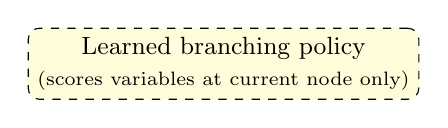
\begin{tikzpicture}
\node[draw, dashed, rounded corners, fill=yellow!15, font=\small, align=center]
{Learned branching policy\\{\scriptsize (scores variables at current node only)}};
\end{tikzpicture}

\caption{Local decision-making in learning to branch. A learned branching policy evaluates only the current node state to score candidate variables and select a branching action. The policy is re-applied independently at each node of the branch-and-bound tree, guiding local tree expansion without explicit evaluation of downstream subtrees.}
\label{fig:learning_to_branch}
\end{figure}
